
\section{Data and Methods}
\label{section:data}

The data comes from the 10\% public use sample of the 2011 South African Census. The micro data at the individual level has observations for each person within a household from all nine provinces of South Africa. I retained only sons or daughters in each household whose biological parents were alive by the time of the census and matched them with data on their mothers. After identifying the order of birth among two or more siblings using their dates of birth, I selected those observations where the age of the firstborn child is less than or equal to 18. Finally, two groups of samples were used in the final analysis. The next subsection discusses these in detail.

\subsection{The 2+ and 3+ Samples}

% latex table generated in R 4.1.2 by xtable 1.8-4 package
% Mon May 16 16:49:34 2022
\begin{table}[t!]
\centering
\caption{Summary Statistics} 
\label{tab:sum-stat}
\begin{tabular}{llrrlrrlrr}
  \toprule
   \\[-1.8ex]  & & \multicolumn{2}{c}{2+ Sample} & & \multicolumn{5}{c}{3+ Sample}  \\[0.2ex] \cline{3-4}  \cline{6-10}  \\[-1.2ex]  & & & & & & & & \multicolumn{2}{c}{First and} \\  & & \multicolumn{2}{c}{Firstborns} & & \multicolumn{2}{c}{Firstborns} & & \multicolumn{2}{c}{Second Borns} \\ \cline{3-4}  \cline{6-7} \cline{9-10}  \\[-1.2ex]  & & \multicolumn{1}{c}{Mean} & \multicolumn{1}{c}{sd} & & \multicolumn{1}{c}{Mean} & \multicolumn{1}{c}{sd} & & 
  \multicolumn{1}{c}{Mean} & \multicolumn{1}{c}{sd} \\  \\[-1.8ex] &  & \multicolumn{1}{c}{(1)} & \multicolumn{1}{c}{(2)} &  & 
  \multicolumn{1}{c}{(3)} & \multicolumn{1}{c}{(4)} &  & 
  \multicolumn{1}{c}{(5)} & \multicolumn{1}{c}{(6)}  \\  \midrule
Number of Children &  & 2.665 & 0.904 &  & 3.592 &  0.87 &  & 3.592 &  0.87 \\ 
  Male &  & 0.499 &  &  & 0.495 &  &  & 0.499 &  \\ 
  Age (Years) &  & 13.14 & 3.061 &  & 14.88 & 2.271 &  & 13.13 & 2.912 \\ 
  Age (Months) &  & 163.1 &  36.8 &  &   184 & 27.18 &  & 162.8 & 34.96 \\ 
  Twins2 &  &  0.01 &  &  &  &  &  &  &  \\ 
  SameSex12 &  & 0.517 &  &  &  &  &  &  &  \\ 
  Boy12 &  & 0.261 &  &  &  &  &  &  &  \\ 
  Girl12 &  & 0.255 &  &  &  &  &  &  &  \\ 
  Twins3 &  &  &  &  & 0.013 &  &  & 0.013 &  \\ 
  SameSex123 &  &  &  &  & 0.274 &  &  & 0.274 &  \\ 
  Boy123 &  &  &  &  & 0.138 &  &  & 0.138 &  \\ 
  Girl123 &  &  &  &  & 0.136 &  &  & 0.136 &  \\ 
  Grade Achieved &  & 6.471 & 2.921 &  & 7.865 & 2.328 &  & 6.386 & 2.761 \\ 
  Educational Attainment &  &     1 & 0.155 &  &     1 & 0.139 &  & 1.002 & 0.159 \\ 
  Left Behind &  & 0.386 &  &  & 0.401 &  &  & 0.376 &  \\ 
  Private School &  & 0.089 &  &  & 0.065 &  &  & 0.063 &  \\ 
  Mother's Age (Years) &  & 36.57 & 5.561 &  & 37.43 & 4.808 &  & 37.43 & 4.808 \\ 
  Age at First Birth &  & 22.94 &  4.86 &  & 22.05 & 4.417 &  & 22.05 & 4.417 \\ 
  Mother in the Labour Force &  & 0.763 &  &  & 0.713 &  &  & 0.713 &  \\ 
  Father in Household &  & 0.608 &  &  & 0.606 &  &  & 0.608 &  \\ 
   \multicolumn{2}{l}{Mother's Population Group} &  &  &  & & & & \\\phantom{M}Black African &  & 0.752 &  &  & 0.819 &  &  & 0.819 &  \\ 
  \phantom{M}Coloured &  & 0.109 &  &  & 0.094 &  &  & 0.094 &  \\ 
  \phantom{M}White &  & 0.107 &  &  & 0.061 &  &  & 0.061 &  \\ 
  \phantom{M}Indian or Asian &  &  0.03 &  &  & 0.023 &  &  & 0.023 &  \\ 
  \phantom{M}Other &  & 0.003 &  &  & 0.003 &  &  & 0.003 &  \\ 
   \multicolumn{2}{l}{Mother's Level of Education} &  &  &  & & & & \\\phantom{M}No schooling &  &  0.05 &  &  & 0.079 &  &  & 0.079 &  \\ 
  \phantom{M}Some Primary &  & 0.089 &  &  & 0.129 &  &  & 0.129 &  \\ 
  \phantom{M}Completed Primary &  & 0.046 &  &  & 0.061 &  &  & 0.061 &  \\ 
  \phantom{M}Some Secondary &  & 0.362 &  &  & 0.391 &  &  & 0.391 &  \\ 
  \phantom{M}Grade 12/Std 10 &  & 0.285 &  &  & 0.224 &  &  & 0.224 &  \\ 
  \phantom{M}Higher &  & 0.168 &  &  & 0.117 &  &  & 0.117 &  \\ 
    \\[-1.8ex] \hline \\[-1.8ex]  \multicolumn{2}{l}{ $ N $ }  &  \multicolumn{2}{c}{94,977} & & \multicolumn{2}{c}{28,679} & & \multicolumn{2}{c}{57,358} \\  \bottomrule   
 \\[-1.8ex] \multicolumn{10}{l}{\footnotesize{\textit{Note:} The standard deviations for proportions is 
               not presented.}} 
\end{tabular}
\end{table}


The 2+ sample consists of only firstborn children with one or more siblings (so the total number of children per mother would be two or more). I selected only firstborns aged 8 to 18.\footnote{ South Africa has a compulsory schooling law where children who have turned 6 by June 30 are required to attend grade 1 (see \url{https://www.education.gov.za/Informationfor/ParentsandGuardians/SchoolAdmissions.aspx}). To look at 8 year olds and above would allow me to observe variations in educational achievement and grade retention. }  The twins IV (Twins2) in this sample is an indicator for whether the second birth was a multiple birth or not. But I have excluded firstborns who are twins themselves because of the special characteristics of twins that could confound results. Hence, all firstborns in this sample are singletons. Similarly, the same sex IV (SameSex12) is an indicator for whether the sex of the first and second births are the same. In order to look at the effect by gender, I disaggregated this into two separate indicators: whether the first two births were both boys (Boy12) or both girls (Girl12).\footnote{ The sum of Boy12 and Girl12 gives the SameSex12 dummy, i.e., SameSex12 = Boy12 + Girl12. }  

The first two columns of \autoref{tab:sum-stat} present summary statistics on the variables in the 2+ sample. The sample consists of almost 95,000 firstborns and has a balanced sex composition. The average number of kids is 2.7 and the mean age of the firstborns is 13. About three-quarters of the observations belong to Black African mothers, while coloured and white mothers each account for approximately 11\%. The rate of occurrence of twins in the second birth is 1\%. On the other hand, about 52\% had a sibling of the same gender from second birth. Given that 50\% of the sample are males, we have an almost equal proportion of matching first two births for each gender: 26.1\% for boys and 25.5\% for girls. 

The 3+ sample is a subsample of the 2+ sample, where both non-twin first and second-born kids with one or more siblings are included. Here also, I selected children aged 8 to 18 since I can only observe variations in schooling outcomes for kids aged 8 or older. The twins IV in this sample (Twins3) is a dummy for whether the third birth was a twin birth or not. The same sex IV, on the other hand, is an indicator for whether the first three kids were of the same sex. This is termed SameSex123. As in the 2+ sample, I have disaggregated this indicator into two separate indicators based on the sex of children in the first three births. The Boy123 and Girl123 are indicators for whether the first three children are all boys or all girls, respectively. 

Columns 3-6 of \autoref{tab:sum-stat} presents summary statistics on the 3+ sample. Columns 3 and 4 focus only on firstborns while columns 5 and 6 include both first and second-borns. There is no substantial difference across many of the variables between the firstborns in the 3+ sample and their counterparts in the 2+ sample. A similar result follows when looking at the entire 3+ sample (i.e., both first and second-borns; $ N = 57,358 $). The average family size in this sample is 3.6 and the average age of the children is 13. Just as in the 2+ sample, we have an almost perfectly balanced sex composition. The twin rate at the third birth, 1.3\%, is a little higher than in the 2+ sample. About 27\% of the observations are in households where the first three births are of the same sex. Again, this is well balanced across the two sexes (about 13.5\% each). Black African mothers now account for a larger proportion (82\%), while the share of white mothers declined to 6.1\%. One can also see that the share of mothers with no schooling is higher in the 3+ sample compared to the 2+ sample (8\% vs. 5\%).   
    

\subsection{Model Specification and Outcome Variables}
\label{section:outcomes}

The structural equation that captures the causal relationship of interest is

\begin{equation}\label{eq:01}
	y_{i} = X_{i}\boldsymbol{\beta} + \gamma n_{i} + \varepsilon_{i}
\end{equation}

where $ y_{i} $ is an outcome variable, $ X_{i} $ is a vector of covariates including characteristics of the children and their mothers, and $ n_{i} $ is the total number of children (including the subject) in the household. As discussed in the introduction, because the number of children, $ n_{i} $, is endogenous, OLS estimation of \eqref{eq:01} gives a biased and inconsistent estimate of $ \gamma $. I use both the birth of twins and the sameness of sex in earlier births to instrument for family size. The rest of the current subsection discusses the outcome variables explored in the study. The next subsection has a detailed discussion on the proposed instruments.  

%\begin{figure}[!htbp]
%\centering
%\caption{\label{fig:hists}Histograms of Educational Attainment Index}
%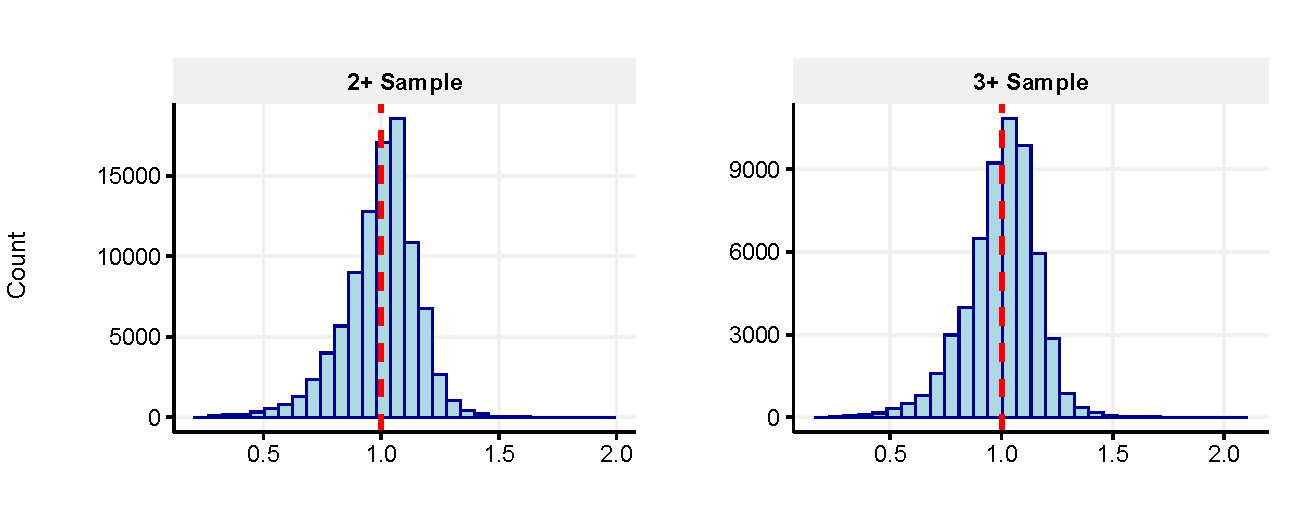
\includegraphics[width=\textwidth]{figures/hists.pdf}
%\end{figure}

The study will look at the effect of sibship size on four outcome variables: (i) educational attainment, (ii) whether a kid is lagging behind in grade, (iii) whether the kid attends a private school, and (iv) the labour force participation of the mother. The first two are final outcome variables whereas the second two are considered as intermediate outcome variables \parencite{caceres-delpiano_impacts_2006}. 

Following \textcite{rosenzweig_testing_1980}, an educational attainment index was constructed by taking the ratio of the highest grade achieved by a child at the time of the census to the mean grade of all kids of the same age, month of birth, and province. The reason month of birth was chosen as a grouping variable is that laws on admission are based on the age of a child at a specific point in time during the admission year.  Hence, the month of birth is one determining factor for the variation in grade achievement of children of the same age. However, individual provinces have their own rules on registration timelines as well as implementation. From \autoref{tab:sum-stat}, the educational attainment index has a mean of 1 and a standard deviation of about 0.16 in both the 2+ and 3+ samples. %\autoref{fig:hists} shows a histogram of this index in both samples, which provides a more informative picture of its distribution. 

Similarly, a dummy for being left behind is constructed by comparing the highest grade of a child to the mode of the highest grade of all kids of the same age, month of birth, and province in the relevant sample. It takes a value of 1 if a child's highest grade is below the mode and 0 if it is equal to or above the mode. This essentially measures the same thing as the educational attainment index but has some advantages over the latter. Particularly, as it uses mode instead of mean, it is not affected by extreme values. But as a discrete measure it does not take into account the extent of the lagging (or progressing). It can be considered as a useful complement to the educational attainment index. According to \autoref{tab:sum-stat}, 38.6\% in the 2+ sample and 37.6\% in the 3+ sample are lagging behind using this measure. 

The third outcome variable, \enquote{private school} is a dummy for whether the child attends a private school ($ = 1 $) or a public school ($ = 0 $). Like in many countries, private schools offer better quality education and are preferred to public schools in South Africa. They are also more expensive. Thus enrollment in private school can reflect costly parental investment in the education of children. Attending a private school can also lead to better educational outcomes. The available evidence suggests that educational outcomes are better for kids attending private school, although we should be careful to interpret this as showing causation, not merely correlation \parencite{caceres-delpiano_impacts_2006}. From \autoref{tab:sum-stat}, about 9\% in the 2+ sample and 6.3\% in the 3+ sample attend private school. These might sound low but are not surprising given that private schools are expensive in South Africa.

The last outcome variable, mothers' labour force participation (Mothers' LFP) is also a dummy for whether a mother is in the labour force ($ =1 $) or not ($ =0 $). The relationship between a mother's labour market outcome and family size has been explored in many studies (\textit{cite a few studies}). As an intermediate outcome, a mother being in the labour force has ambiguous effects on child outcomes \parencite{caceres-delpiano_impacts_2006}. On the one hand, working mothers generate income that they can invest on their children, but, on the other hand spend less time caring for their children. Either way, it is an important channel between fertility and the welfare of children. According to Table 1, about 76.3\% of mothers were in the labour force in the 2+ sample, while the corresponding figure in the 3+ sample is 71.3\%.


\subsection{Instrumental Variables, Interpretation, and First Stages}
\label{section:IVs}

The main motivation behind the use of instrumental variables is to uncover a causal relationship between family size and outcomes for children. Following the potential outcomes framework, what we are trying to estimate using the birth of twins and the sex composition of siblings as natural experiments is what \textcite{Angrist1995} called the Average Causal Response (ACR). \textcite{Angrist1995} have shown that, given mild regularity assumptions, the Two Stages Least Squares (2SLS) estimates using a binary instrument $ Z $ to instrument for an endogenous variable that takes a finite set of integer values  (say $ 0, 1, \dots, J $) is the weighted average of per-unit causal effects (that is, the effect of going from 0 to 1, the effect of going from 1 to 2, and so on) along the length of an appropriately defined causal response function. ...

% Consider shortening/removing this paragraph if necessary.
%The other important assumption needed to estimate the ACR is monotonicity. To understand the idea behind this assumption, we need to introduce the four mutually exclusive groups comprising of our quasi-experimental population: compliers, always takers, never takers, and defiers. These were first outlined in the treatment-effects framework of \textcite{angrist_identification_1996}.  Always takers always get treated regardless of their assignment, never takers never get treated regardless of their assignment, and compliers get treated when the instrument is switched on and don't get treated otherwise. The defiers, on the other hand, are a very strange group who get treated when the instrument is switched off and don't get treated when it is switched on. The assumption of monotonicity rules out the presence of defiers since they complicate the link between ACR and the reduced form \parencite{Angrist2009}.\footnote{\textcite{Angrist2009} discuss monotonicity in the context of the LATE framework of \textcite{imbens_identification_1994}. But this carries over directly to the ACR since the ACR is just an extension of the LATE \parencite[see][p.~181]{Angrist2009}.}  In other words, monotonicity rules out the case where the instrument pushes some people into treatment while pushing others out. In our case, monotonicity requires that the proposed instrument moves fertility in one direction only. In particular, we assume that the potential number of children when the instrument is switched on is at least as large as it would have been when it is switched off; i.e., $ N_{1i} \geq N_{0i} $. This is automatically satisfied by the twins instrument as fertility is always increased because of a twin birth for any mother. However, monotonicity need not hold for the same sex instrument as there could be parents who prefer children of the same sex and therefore go on to have another child if the sexes of the first two or three children are different \parencite{Huber2015}. In Section~\ref{section:samesx}, I discuss a partial check for monotonicity using first stage regressions. 



\subsubsection{The Twins Instrument}

%The first stage for the twins instrument is
%
%\begin{equation}\label{eq:05}
%	n_{i} = X_{i}\boldsymbol{\theta} + \delta\cdot {\rm Twins }_{i} + \xi_{i}
%\end{equation}

The twins IV used in this study is an indicator for the occurrence of twins in the second (Twins2) or third (Twins3) birth, corresponding to the 2+ and 3+ samples, respectively.\footnote{There are two rationales for considering twins at a fixed parity and looking at outcomes for older non-twin children. First, it accounts for the fact that twins are more likely in a larger family. Second, looking at older children before the twin birth avoids the confounding effect from birth order that would occur after a twin birth \parencite{Black2010}. The obvious drawback of focusing on children prior to the occurrence of twins is that it doesn't allow us to look at the effect on the marginal child.} Column 1 of \autoref{tab:frst-stage} reports the first stage results for the twins instruments. The results clearly show that, in both the 2+ and 3+ samples, the occurrence of twins significantly increases the number of children. A twin second birth increases the number of children by 0.83 whereas a twin third birth leads to 0.76 additional children, controlling for the other covariates in the model. These estimates remain virtually the same after controlling for same sex dummies by gender (column 4).  The twins instrument is also relevant in both samples as evident from the sufficiently large F statistics from the Wald test (963 for the 2+ sample; 484 for the 3+ sample), ruling out the case of weak instruments.


%Tex File: D:/R_projects/MScED_Dissertation/tex/tables/frst-stage.tex

% Date and time: Fri, May 13, 2022 - 2:54:47 PM
\begin{table}[!htbp] \centering 
  \caption{First Stage Regressions} 
  \label{tab:frst-stage} 
\begin{threeparttable}
\begin{tabular}{@{\extracolsep{5pt}}lcccc} 
\\[-1.8ex]\hline 
\hline \\[-1.8ex] 
 & \multicolumn{4}{c}{\textit{Dependent variable:}} \\ 
\cline{2-5} 
\\[-1.8ex] & \multicolumn{4}{c}{Number of Children} \\ 
\\[-1.8ex] & (1) & (2) & (3) & (4)\\ 
\hline \\[-1.8ex] 
\\[-2.0ex] \multicolumn{5}{@{} l}{\textbf{Panel A: 2+ Sample}}
 \\
 \\[-1.5ex]
 Twins2 & 0.830$^{***}$ &  &  & 0.830$^{***}$ \\ 
  & (0.027) &  &  & (0.027) \\ 
  & & & & \\ 
 SameSex12 &  & 0.037$^{***}$ &  &  \\ 
  &  & (0.005) &  &  \\ 
  & & & & \\ 
 Boy12 &  &  & 0.016$^{**}$ & 0.015$^{**}$ \\ 
  &  &  & (0.008) & (0.008) \\ 
  & & & & \\ 
 Girl12 &  &  & 0.057$^{***}$ & 0.057$^{***}$ \\ 
  &  &  & (0.008) & (0.007) \\ 
  & & & & \\ 
\cline{2-5} \\[-2.0ex]
F & 962.7 & 47.38 & 31.02 & 342. \\ 
Observations & 94,977 & 94,977 & 94,977 & 94,977 \\ 
R$^{2}$ & 0.184 & 0.177 & 0.177 & 0.185 \\ 
\\[-1.83ex] 
 \hline \\[-1.83ex]
\\[-2.0ex] \multicolumn{5}{@{} l}{\textbf{Panel B: 3+ Sample}}
 \\
 \\[-1.5ex]
 Twins3 & 0.761$^{***}$ &  &  & 0.762$^{***}$ \\ 
  & (0.035) &  &  & (0.035) \\ 
  & & & & \\ 
 SameSex123 &  & 0.051$^{***}$ &  &  \\ 
  &  & (0.011) &  &  \\ 
  & & & & \\ 
 Boy123 &  &  & 0.018 & 0.019 \\ 
  &  &  & (0.014) & (0.014) \\ 
  & & & & \\ 
 Girl123 &  &  & 0.083$^{***}$ & 0.084$^{***}$ \\ 
  &  &  & (0.015) & (0.015) \\ 
  & & & & \\ 
\cline{2-5} \\[-2.0ex]
F & 484.1 & 22.19 & 15.95 & 172.3 \\ 
Observations & 57,358 & 57,358 & 57,358 & 57,358 \\ 
R$^{2}$ & 0.152 & 0.143 & 0.143 & 0.153 \\ 
\\[-2.0ex]
\hline 
\hline \\[-1.8ex] 
\end{tabular} 
\begin{tablenotes}
\footnotesize
\item \textit{Notes:} Covariates for all regressions include age (in months) and sex of child, 
mother's characteristics, dummies for districts, and a dummy for whether the father resides in the household.
The regressisons for the 3+ sample in addition include dummies for birth order. F statistics are from the Wald 
test for exclusion restrictions of the relevant instrument(s) from the regression. Robust standard errors 
(for the 2+ sample) and cluster robust standard errors (for the 3+ sample; clustered by mother's ID) are in parenthesis. 
*** Significant at 1\%, ** Significant at 5\%, * Significant at 10\%.
\end{tablenotes}
\end{threeparttable}
\end{table} 



 

It is important to point out what we can learn from the first stage of the twins instrument. The ACR framework introduced [in Addendum] offers two important insights on the twins identification strategy. First, the twins instrument captures the causal effect of having children on a narrow range \parencite{angrist_multiple_2010}. This is because the weights used in the calculation of $ \beta_{w} $ in \eqref{eq:02} rapidly decline with the number of births as the first stage gets weaker at higher parities. This is shown in Panel A of \autoref{fig:02}, which plots the first stage estimates, along with their 95\% confidence intervals, of the twin IVs (Twins2 and Twins3) on dummies for having at least $ j $ kids $ (j = 3, 4, \dots, 9) $.\footnote{ The coefficients and standard errors are obtained by running a simple linear regression of a dummy for having at least $ j $ kids $ (j = 3, 4, \dots, 9) $ on the twins instruments (Twins2 and Twins3). The coefficients plotted provide an estimate of $ \mathbb{P}(N_{1i} \geq j > N_{0i}) $ for $ j = 3, 4, \dots, 9 $ and their sum is equal to the (unconditional) first stage coefficient (see \eqref{eq:04}). } The first stage effects of both instruments decline sharply with more births. For example, having twins in the third birth increases the likelihood of having at least 4 kids by 0.6 while it increases the likelihood of having 5 or more kids by 0.1, with much smaller effects for 6 or more kids and no significant effects above that.  The implication of this is that the twins instrument \enquote{captures an average causal effect over a range of fertility variation that is close to the parity of the multiple birth} \parencite[p.~788]{angrist_multiple_2010}. 

%\begin{singlespace}
%
%Tex File: D:/R_projects/MScED_Dissertation/tex/tables/frst-stage.tex

% Date and time: Fri, May 13, 2022 - 2:54:47 PM
%\begin{table}[!htbp] \centering 
\begin{wraptable}{L}{10.5cm}
  \caption{First Stage Regressions} 
  \label{tab:frst-stage} 
\begin{singlespace}
\begin{threeparttable}
\begin{tabular}{@{\extracolsep{5pt}}lcccc} 
\\[-1.8ex]\hline 
\hline \\[-1.8ex] 
 & \multicolumn{4}{c}{\textit{Dependent variable:}} \\ 
\cline{2-5} 
\\[-1.8ex] & \multicolumn{4}{c}{Number of Children} \\ 
\\[-1.8ex] & (1) & (2) & (3) & (4)\\ 
\hline \\[-1.8ex] 
\\[-2.0ex] \multicolumn{5}{@{} l}{\textbf{Panel A: 2+ Sample}}
 \\
 \\[-1.5ex]
 Twins2 & 0.830$^{***}$ &  &  & 0.830$^{***}$ \\ 
  & (0.027) &  &  & (0.027) \\ 
  & & & & \\ 
 SameSex12 &  & 0.037$^{***}$ &  &  \\ 
  &  & (0.005) &  &  \\ 
  & & & & \\ 
 Boy12 &  &  & 0.016$^{**}$ & 0.015$^{**}$ \\ 
  &  &  & (0.008) & (0.008) \\ 
  & & & & \\ 
 Girl12 &  &  & 0.057$^{***}$ & 0.057$^{***}$ \\ 
  &  &  & (0.008) & (0.007) \\ 
  & & & & \\ 
\cline{2-5} \\[-2.0ex]
F & 962.7 & 47.38 & 31.02 & 342. \\ 
Observations & 94,977 & 94,977 & 94,977 & 94,977 \\ 
R$^{2}$ & 0.184 & 0.177 & 0.177 & 0.185 \\ 
\\[-1.83ex] 
 \hline \\[-1.83ex]
\\[-2.0ex] \multicolumn{5}{@{} l}{\textbf{Panel B: 3+ Sample}}
 \\
 \\[-1.5ex]
 Twins3 & 0.761$^{***}$ &  &  & 0.762$^{***}$ \\ 
  & (0.035) &  &  & (0.035) \\ 
  & & & & \\ 
 SameSex123 &  & 0.051$^{***}$ &  &  \\ 
  &  & (0.011) &  &  \\ 
  & & & & \\ 
 Boy123 &  &  & 0.018 & 0.019 \\ 
  &  &  & (0.014) & (0.014) \\ 
  & & & & \\ 
 Girl123 &  &  & 0.083$^{***}$ & 0.084$^{***}$ \\ 
  &  &  & (0.015) & (0.015) \\ 
  & & & & \\ 
\cline{2-5} \\[-2.0ex]
F & 484.1 & 22.19 & 15.95 & 172.3 \\ 
Observations & 57,358 & 57,358 & 57,358 & 57,358 \\ 
R$^{2}$ & 0.152 & 0.143 & 0.143 & 0.153 \\ 
\\[-2.0ex]
\hline 
\hline \\[-1.8ex] 
\end{tabular} 
\begin{tablenotes}
%\begin{singlespace}
\footnotesize
\item \textit{Notes:} Covariates for all regressions include age (in months) and sex of child, 
mother's characteristics, dummies for districts, and a dummy for whether the father resides in the household.
The regressisons for the 3+ sample in addition include dummies for birth order. F statistics are from the Wald 
test for exclusion restrictions of the relevant instrument(s) from the regression. Robust standard errors 
(for the 2+ sample) and cluster robust standard errors (for the 3+ sample; clustered by mother's ID) are in parenthesis. 
*** Significant at 1\%, ** Significant at 5\%, * Significant at 10\%.
%\end{singlespace}
\end{tablenotes}
\end{threeparttable}
\end{singlespace}
\vspace{-30pt}
\end{wraptable} 




 
%\end{singlespace}

The second noteworthy feature of the twins IV is that it captures the causal effect of fertility for non-treated families, i.e., families who didn't experience a multiple birth at the specified parity. In the ACR framework (or the LATE framework, in general), with the monotonicity assumption in place, the treated consist of the compliers and always takers and the non-treated consist of the compliers and never takers.\footnote{ There are four mutually exclusive groups comprising of our quasi-experimental population: compliers, always takers, never takers, and defiers. These were first outlined in the treatment-effects framework of \textcite{angrist_identification_1996}. Always takers always get treated regardless of their assignment, never takers never get treated regardless of their assignment, and compliers get treated when the instrument is switched on and don't get treated otherwise. The defiers, on the other hand, are a very strange group who get treated when the instrument is switched off and don't get treated when it is switched on. The assumption of monotonicity rules out the presence of defiers since they complicate the link between ACR and the reduced form \parencite{Angrist2009}. } An instrument \enquote{is not informative about effects on never-takers and always-takers because, by definition, treatment status for these two groups is unchanged by the instrument} \parencite[p.~158]{Angrist2009}. Hence, instruments do not usually capture the average causal effect on all of the treated or on all of the non-treated. But there are no never takers when it comes to the twins instrument since all women who have a twins second (third) birth end up with at least three (four) children. Therefore, \enquote{the parameter identified by twins instruments is the average effect on the non-treated.} \parencite[p.~788]{angrist_multiple_2010}.



\subsubsection{The Same Sex Instrument}
\label{section:samesx}

The rationale for using the gender composition of siblings as an IV is based on the widely observed phenomenon of parental preferences for a mixed sibling-sex composition and that sex mix is virtually randomly assigned \parencite{angrist_children_1998}. There is plenty of empirical support for the claim that parents prefer to have children of both genders and that this preference drives the decision to have additional children \parencite[e.g.,][]{norling_measuring_2018,bisbee_local_2015}. The first stage regression on the same sex dummies is also consistent with this observation. Column 2 of \autoref{tab:frst-stage} shows that, in both the 2+ and 3+ samples, the same sex dummy has a positive and statistically significant effect on the number of children.  The first stage effects of SameSex12 (in the 2+ sample) and SameSex123 (in the 3+ sample) is 0.037 and 0.051, respectively, and both are statistically significant at the 1\% level. The first stage results of the same sex dummies when disaggregated by gender reveal an interesting pattern. For the 2+ sample, the first stage effect of having two girls (0.057) is about three and a half times as large as the corresponding effect of having two boys (0.016). This gets even more pronounced in the 3+ sample: while having three boys has no statistically significant effect on the number of children, having three girls increases family size by 0.083 and the effect is statistically significant at the 1\% level of significance. It seems childbearing increases in response to having only girls more than having only boys.\footnote{ This might reveal sex preference dynamics in favour of boys, a subject which is not explored in this study. } 

The results obtained using the same sex IV should also be interpreted as an average causal response (ACR) that applies only to the subpopulation of compliers--- i.e., those families whose number of children was increased because of having had two (three) first children of the same sex. However, the ACR here differs from the one captured by the twins instrument in two important ways \parencite{angrist_multiple_2010}. First, the complier population is less than complete; not all of the non-treated are affected by the instrument. In other words, there could well be never takers, those that would not have any more children whether treated or not, among the non-treated. Second, the sex composition instrument drives fertility over a wider range of parities than the twins instrument. This is shown in Panel B of \autoref{fig:02}, which plots the first stage effects of a same-sex sibling composition on having $ j $ or more kids $ (j = 3, 4, \dots, 9) $, similar to the first stage effects discussed for the twins instruments in Panel A earlier. The effect of a same-sex sibship declines less sharply with the number of kids when compared with the corresponding effects of twin births (Panel A). This is particularly true in the 3+ sample. Panels C and D of \autoref{fig:02} plot the first stage effects of an all-male or an all-female sex composition. The plots make it is clear that the positive effect of a same-sex sibship on family size is driven by an all-girls sibship as opposed to having only boys. This suggests that an all-female sibship induces some families to keep having children at higher parities in order to achieve a more balanced sex composition. 

%This is particularly true for the Girl12 and Girl123 instruments. Panels B and C of \autoref{fig:02} show the first stage effects of an all male or an all female sex composition on having $ j $ or more kids $ (j = 3, 4, \dots, 9) $, similar to the first stage effects discussed for the twins instruments in Panel A earlier. The plots make it is clear that the positive effect of same sex sibship on family size is driven by an all-girls sibship as opposed to having only boys. More importantly, the effect of an all female sibship declines less sharply with the number of kids in both the 2+ and 3+ samples, when compared with the corresponding effects of twin births (Panel A). This suggests that an all-female sibship induces some families to keep having children at higher parities in order to achieve a more balanced sex composition. 

%Another issue that needs to be addressed is the possibility that the monotonicity assumption could be violated when using sex composition instruments. This is because, as discussed above, we cannot rule out the presence of defiers. As a partial check on monotonicity, I estimated the same sex first stage in the 2+ sample for each combination of the mother's population group, intervals of the mother's age at first birth, and the level of education of the mother. The results of the unconditional first stages along with their 95\% confidence intervals are plotted in \autoref{fig:03}. As shown in Panel A, out of the 44 first stage regressions, corresponding to the 44 cells, only three generate negative estimates and all three are insignificant.\footnote{ I omitted 4 cells with less than 50 observations in them. } Panels B and C show the corresponding results for the Boy12 and Girl12 instruments, respectively. The results for Girl12 are similar to that of SameSex12, and the first stage effect is stronger than for Boy12 in each cell. The results for Boy12 are less robust and contains more number of negative estimates. But only two of the negative estimates are marginally significant at the 5\% level, while the rest are insignificant. Overall, the results give no indication for the presence of defiers whose fertility decision is negatively impacted by same-sex siblings in earlier births.






